\documentclass[12pt,a4paper,catalan]{article}
\usepackage[utf8]{inputenc}
\usepackage[catalan]{babel}
\usepackage{amsmath}
\usepackage{amsfonts}
\usepackage{amssymb}
\usepackage{graphicx}
\usepackage{float}
\usepackage{framed}
\usepackage{url}
\graphicspath{{images/}}
\usepackage[backend=biber,style=numeric,citestyle=numeric]{biblatex}
\addbibresource{bibliography.bib}
\author{Marc Ferrer Fontirroig}
\title{Rehabilitació complementària basada en videojocs utilitzant Leap Motion}
\begin{document}
	\thispagestyle{empty}
	\begin{center}
		
\includegraphics{uib-logo.jpg}
	\end{center}
	\begin{center}
		\textbf{ESCOLA POLITÈCNICA SUPERIOR}\\
		\textbf{UNIVERSITAT DE LES ILLES BALEARS}\\
		\vspace{2em}
		\textbf{PROJECTE FINAL DE CARRERA}\\
		\vspace{1.5em}
		\textbf{ESTUDIS:}
		\begin{framed}
			\textbf{ENGINYERIA INFORMÀTICA}
		\end{framed}
		\textbf{TÍTOL}
		\begin{framed}
			\textbf{REHABILITACIÓ COMPLEMENTÀRIA BASADA EN VIDEOJOCS UTILITZANT LEAP MOTION}
		\end{framed}
		\vspace{1.7em}
	\end{center}
	\begin{flushright}
		\textbf{Autor:} Marc Ferrer Fontirroig\\
		\textbf{Directora:} Cristina Manresa Yee\\
	\end{flushright}
	\textbf{Data:} Juny 2017
	\newpage
	\tableofcontents
	\newpage
	\listoffigures
	\newpage
	\section{Introducció}
	\subsection{Motivació}
	\subsection{Objectius}
	L'objectiu principal d'aquest projecte fi de carrera, és realitzar una prova de concepte d'exercicis de rehabilitació de lesions de les articulacions de la mà (canell i dits) utilitzant interfícies basades en visió comercials.
	
	La utilització d'exercicis basats en videojocs, aporta un context motivacional extra que pot ajudar a augmentar la participació dels usuaris en la seva teràpia de rehabilitació, tant en temps invertit, com en quant a l'atenció a aquests exercicis. Això és un aspecte fonamental per a l'èxit de la rehabilitació.
	
	La teràpia remota basa da en videojocs presenta un desavantatge, i és la falta de supervisió per part del responsable de la rehabilitació, típicament un fisioterapeuta.
	
	Per tal de suplir aquest desavantatge un dels objectius d'aquesta prova de concepte és que les aplicacions és que el responsable de la teràpia sigui capaç de veure una reproducció dels moviments realitzats per l'usuari. D'aquesta manera es pot fer un seguiment de l'evolució de l'usuari més de manera més ràpida. De la mateixa manera el responsable de la teràpia és capaç de detectar possibles errors en la realització dels exercicis de rehabilitació, que d'una altra manera podrien tenir un efecte perjudicial per l'usuari, i aquests es poden corregir de manera gairebé immediata.
	
	En concret, es pretén utilitzar el controlador Leap Motion. El Leap Motion, és un dispositiu capaç de detectar i capturar les dades de les mans i els dits dins el seu camp de visió, sense necessitat d'utilització de cap tipus de marca de referència. Tot i que no està específicament dissenyat per a rehabilitació, el seu preu reduït i les seves dimensions en comparació a altres dispositius de visió, fan que aquest sigui un dispositiu idoni per els tipus d'exercicis proposats.
	\section{Treballs relacionats}
	\section{Anàlisi i disseny}
	\subsection{Introducció}
	\indent Dins aquest apartat s'analitza i descriu quin ha estat el sistema desenvolupat per tal de satisfer els objectius plantejats anteriorment.
	
	En primer lloc es presenta una descripció de l'arquitectura i les caracterís-tiques del controlador Leap Motion.
	
	Posteriorment es fa una anàlisi de requisits del sistema a desenvoluapar tant des del punt de vista fucional com tecnològic, la qual cosa permet tenir una descripció detallada del sistema.
	
	Com a darrera secció es descriu el disseny de l'aplicació amb tots els seus subsistemes i els diferents jocs desenvolupats, així com els seus detalls d'implementació.
	
	\subsection{Leap motion}
	El Leap motion és un dispositiu petit dispositiu que es connecta mitjançant USB i que és capaç de capturar els moviments de mans i dits, així com gestos i com petits objectes com llapis. Per fer-ho utilitza dues càmeres i tres LEDs infrarojos, el dispositiu és capaç de capturar les dades de les mans fins a una distància d'uns 60cm, tant a la part superior com als laterals del dispositiu, gràcies al gran camp de visió de les càmeres  \cite{leapcharacteristics}.
	\begin{figure}[H]
		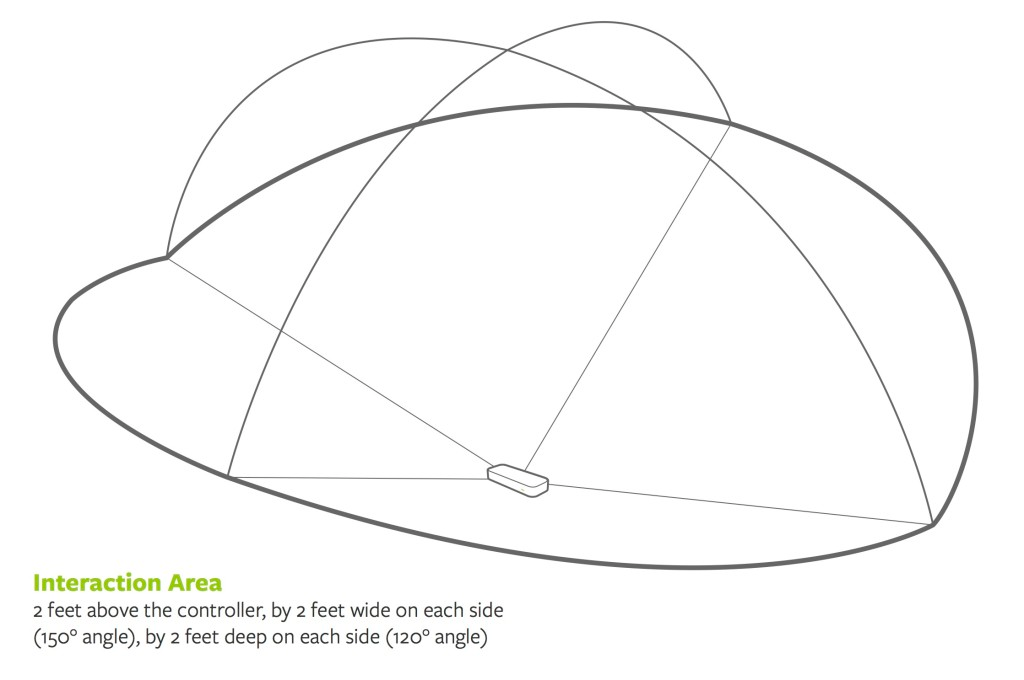
\includegraphics[width=\textwidth,keepaspectratio]{leap-motion-interaction-area.png}
		\centering
		\caption{Representació del dispositiu i el seu camp de visió \protect\cite{leapcharacteristics}}
	\end{figure}
	Les dades capturades per aquestes càmeres són enviades per USB al ordinador al qual es connecta el controlador Leap, on el software de Leap Motion, que s'executa com un servei, s'encarrega de processar-les i deixar-les disponibles per a que puguin ser obtingudes mitjançant APIs.
	El servei del Leap Motion proporciona la informació a les APIs en forma d'una sèrie de fotogrames que contenen tota la informació de seguiment capturada. Al final és competència de d'aquestes APIs proporcionar a l'usuari les dades en forma d'estructures orientades a objectes, així com també proporcionar una sèrie de funcions que permeten operar amb aquestes dades.
	
	\subsubsection{Arquitectura del Leap Motion}
	El Leap Motion és capaç de funcionar en múltiples sistemes operatius i les seves dades poden ser obtingudes de dues formes; mitjançant una interfície nativa o a través d'un servidor de Web socket. D'aquesta manera, les possibilitats per als desenvolupadors són molt diverses i inclouen molts dels llenguatges de programació més utilitzats actualment \cite{leapsdkdocs}.
	
	\paragraph{Interfície nativa}
	La interfície nativa es proporciona a través d'una llibreria que connecta el servei del Leap Motion. Aquest servei després proveeix les dades de seguiment obtingudes a les apliacions desenvolupades. La llibreria es pot utilitzar directament en el cas d'aplicacions desenvolupades amb C++ i Objective C, o es poden utilitzar una de les APIs per Java, C\# o Python \cite{leapsdkdocs}.
	
	\begin{figure}[H]
		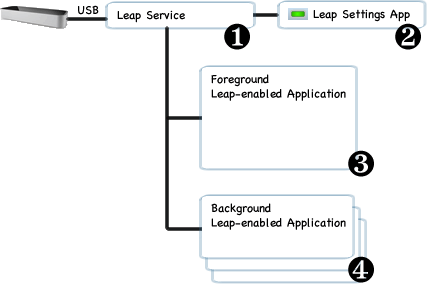
\includegraphics[width=\textwidth,keepaspectratio]{native-interface.png}
		\centering
		\caption{Esquema d'aplicacions utilitzant la interfície nativa.}
	\end{figure}
	\begin{enumerate}
		\item El servei de Leap Motion rep les dades del controlador a través d'una connexió USB, processa les dades rebudes i les envia a les aplicacions. Per defecte el servei només envia informació a les aplicacions en primer pla, però les aplicacions poden demanar rebre dades també en segon pla.
		\item L'aplicació de Leap Motion és independent del servei i permet als usuaris configurar la seva instal·lació de Leap Motion.
		\item Una aplicació en primer pla rep dades de seguiment del servei de Leap Motion.
		\item Quan una aplicació perd el focus del sistema operatiu, el servei de Leap Motion deixa d'enviar-li dades. Les aplicacions dissenyades per funcionar en segon pla poden demanar al servei que els proveeixi dades de seguiment fins i tot en segon pla.
	\end{enumerate}
	
	\paragraph{Interfície web socket}
	El servei de Leap Motion executa un servidor de web socket local en el domini local (localhost) a través del port 6437. Aquesta interfície de web socket proveeis dades de seguiment en format JSON. Després un client JavaScript desenvolupat per la mateix empresa de Leap Motion, s'encarrega de capturar aquestes dades i presentar-les com a objectes de JavaScript estàndard.
	
	\begin{figure}[H]
		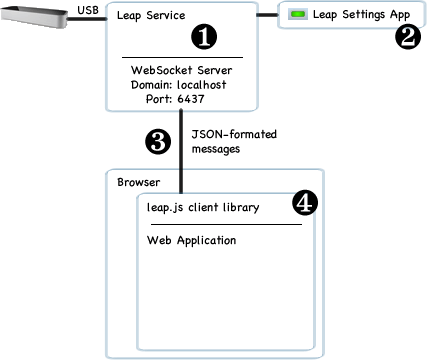
\includegraphics[width=\textwidth,keepaspectratio]{websocket-interface.png}
		\centering
		\caption{Esquema d'aplicacions utilitzant la interfície de web socket.}
	\end{figure}
	
	\begin{enumerate}
		\item El servei de Leap Motion proveeix un servidor de web socket a través de la direcció http://127.0.0.1:6437.
		\item L'apliació de configuració del Leap Motion permet habilitar o deshabilitar el servidor de web socket.
		\item El servidor envia les dades de seguiment en format JSON. Les aplicacions també poden enviar missatges de configuració al servidor.
		\item La mateixa empresa de Leap Motion ens proveeix d'una llibreria JavaScript que pot ser utilitzada per les aplicacions web per accedir a les dades de seguiment del Leap Motion.
	\end{enumerate}
	
	Aquesta interficie està dissenyada per ser utilitzada per aplicacions web, tot i que qualsevol aplicació pot establir una connexió amb el servidor de web socket. Aquest servidor segueix l'estàndard de web socket RFC6455

	\subsection{Requeriments}
	Tot i l'objectiu principal del projecte és realitzar una prova de concepte per confirmar que és possible utilitzar el controlador Leap Motion per complementar i monitoritzar teràpies de rehabilitació, és important establir una sèrie de requeriments tècnics i funcionals del projecte per tal de definir bé el seu abast.
	\subsubsection*{Requeriments d'usuari}
	\begin{description}
		\item [RU1] Un usuari ha de poder seleccionar un exercici a realitzar d'una llista.
		\item [RU2] Un usuari ha de poder realitzar exercicis d'extensió del canell.
		\item [RU3] Un usuari ha de poder realitzar exercicis d'abducció i adducció del canell.
		\item [RU4] Un usuari ha de poder realitzar exercicis d'abducció i adducció dels dits.
		\item [RU5] Un Responsable de la rehabilitació d'un usuari ha de ser capaç de reproduir les sessions d'exercicis dels usuaris.
	\end{description}
	\subsubsection*{Requeriments funcionals}
	\begin{description}
		\item [RF1] Els jocs han de ser el més intuïtius possibles.
		\item [RF2] Els jocs han d'engrescar als usuaris a realitzar els exercicis.
		\item [RF3] Els jocs han d'enviar les dades de seguiment dels moviments.
		\item [RF4] Cada joc ha de permetre als usuaris realitzar un sol exercici.
	\end{description}
	\subsubsection*{Requeriments no funcionals}
	\begin{description}
		\item [RNF1] Els jocs han de poder ser executats a qualsevol sistema operatiu.
		\item [RNF2] Els usuaris no han d'instal·lar cap applicació addicional llevat dels controladors del dispositiu Leap Motion.
	\end{description}
	\subsection{Arquitectura del sistema}
	Una vegada definits els requeriments del projecte, a continuació es presenta una descripció de l'arquitectura dissenyada per tal de satisfer aquests requeriments.
	
	Un dels objectius ha estat des del primer moment que l'accés a l'aplicació fos el més fàcil possible per part dels usuaris. Per això es va decidir que el millor era que les aplicacions s'executassin en un entorn web.
	
	Una aplicació web te l'avantatge de ser multiplataforma, és independent del sistema operatiu que tingui l'usuari el qual facilita l'accés a l'aplicació.
	
	En el nostre cas s'utilitza una una arquitectura web tradicional que consta d'un servidor web que és l'encarregat de servir les aplicacions de rehabilitació als usuaris. Aquestes aplicacions contenen la major part de la lògica de l'aplicació. L'arquitectura presenta una peculiaritat, fora del que és una aplicació web tradicional, que és l'utilització d'un servidor de web socket és l'encarregat de rebre les dades del dispositiu Leap Motion dels usuaris i guardar aquestes dades en fitxers per a que puguin ser reproduïts posteriorment pels responsables de les terapies de rehabilitació.\\
	
	// grafic de l'arquitectura de l'aplicació
	
	\begin{description}
		\item [Aplicacions web de rehabilitació] aquestes aplicacions són les encarregades de connectar-se al dispositiu Leap Motion dels usuaris per tal que aquests puguin realitzar els exercicis.
		\item [Servidor web] Un servidor web tradicional encarregat de servir les pagines web als usuaris. També ha de ser l'encarregat de gestionar totes les dades dels usuaris per a que els responsables de la teràpia puguin fer un seguiment de les sessions de rehabilitació dels usuaris.
		\item [Servidor web socket] és un servidor que habilita una comunicació bidireccional en temps real amb els usuaris. Aquest servidor s'encarrega de guardar les dades enviades pels dispositius Leap Motion dels usuaris per tal que aquestes puguin ser monitoritzades posteriorment.
		\item [Base de Dades] ?????????????????????????????
	\end{description}
	\subsection{Disseny dels jocs}
	Per tal de satisfer els requeriments plantejats anteriorment, s'han dissenyat tres jocs diferents.\\
	Cada joc està dissenyat per treballar un tipus d'exercici determinat. Això implica que la complexitat del joc no pot ser molt elevada, ja que el control que pot arribar a tenir l'usuari sobre el joc, realitzant una mateixa acció repetidament és baix. A més, no s'ha d'oblidar que l'objectiu principal dels jocs no és el simple entreteniment de l'usuari, sinó que el més important és que l'usuari es senti motivat per realitzar els exercicis de rehabilitació i els realitzi de manera correcte.\\
	A més s'ha desenvolupat una aplicació de monitorització, que podria ser utilitzada pels responsables de de la rehabilitació per dur a terme un seguiment de l'evolució dels usuaris.
	\subsubsection{Runner boy - Exercici d'extensió del canell}
	Aquest joc està específicament dissenyat per treballar el moviment d'extensió del canell.
	És un joc de desplaçament lateral infinit on l'usuari agafa el control d'una persona o jugador, que va corrent per l'escenari del joc com es mostra a la figura \ref{fig:runnerboy-simple}.
	\begin{figure}[H]
		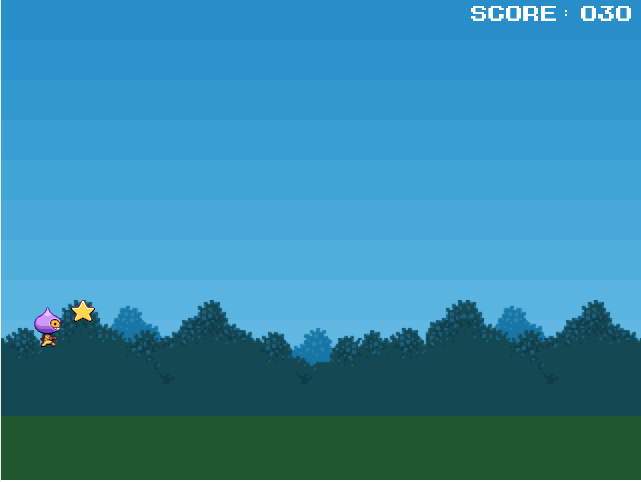
\includegraphics[width=0.8\textwidth,keepaspectratio]{runner-boy-simple.png}
		\centering
		\caption{Imatge del jugador saltant per capturar una estrella.}
		\label{fig:runnerboy-simple}
	\end{figure}
	L'objectiu és capturar unes estrelles que van apareixent en direcció contraria a l'usuari per obtenir punts. Per tal d'afegir complexitat al joc també apareixen uns obstacles que l'usuari ha d'esquivar per no perdre la partida. A més a mesura que la puntuació de l'usuari es va incrementant, també ho fa la velocitat a la que es desplaça el joc, tant els obstacles com les estrelles de puntuació.
	L'usuari controla el joc per mitjà del dispositiu Leap Motion. El primer té la capacitat de fer botar el jugador, per tal d'obtenir les estrelles que s'acosten per l'aire o d'esquivar els obstacles que apareixen per terra, tal com es mostra a la figura \ref{fig:runnerboy-obstacle}.
	\begin{figure}[H]
		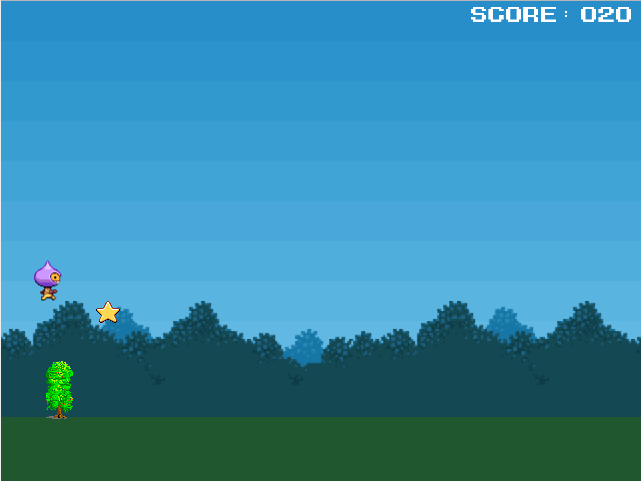
\includegraphics[width=0.8\textwidth,keepaspectratio]{runner-boy-obstacle.png}
		\centering
		\caption{Imatge del jugador esquivant un obstacle durant la partida.}
		\label{fig:runnerboy-obstacle}
	\end{figure}
	El jugador realitza el moviment de salt quan l'usuari estén el canell, elevant els dits de la mà per sobre del canell tant com li sigui possible.
	\subsubsection{Cubes road - Exercici d'abducció i adducció del canell}
	En aquest joc, els usuaris treballen els moviments d'abducció i adducció del canell de la mà. Es tracte d'un joc en 3 dimensions, en el que uns cubs es mouen a través d'una carretera en direcció a l'usuari, aquest ha d'intentar capturar-los desplaçant lateralment un altre cub.
	
	L'objectiu del joc és capturar la major quantitat de cubs possibles, incrementant així la puntuació de l'usuari. A mesura que la puntuació de l'usuari augmenta, també ho fa la velocitat a la que es desplacen els objectes cap a ell augmentant així la dificultat del joc.
	\begin{figure}[H]
		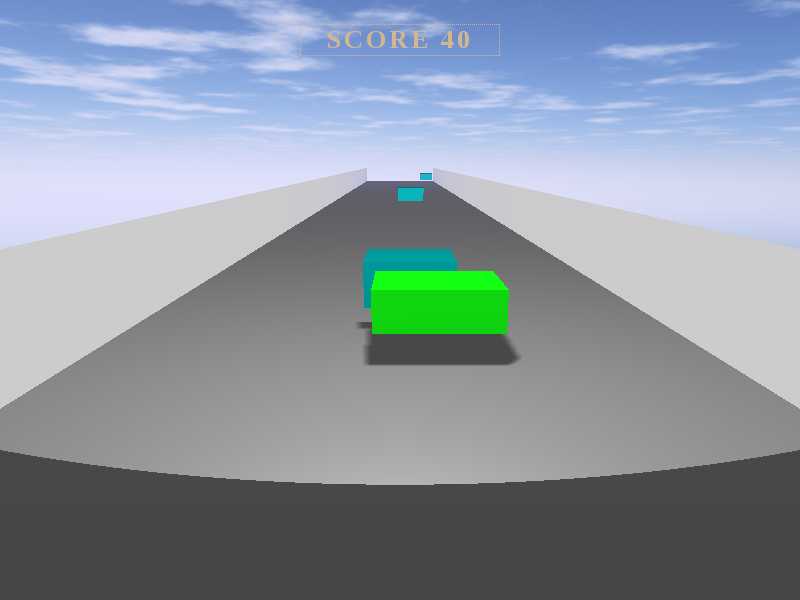
\includegraphics[width=0.8\textwidth,keepaspectratio]{cubes-road-simple.png}
		\centering
		\caption{Situació normal del joc.}
		\label{fig:cubes-road-simple}
	\end{figure}
	Amb l'objectiu d'augmentar la complexitat del joc i la motivació dels usuaris, periòdicament van apareixent uns cubs d'un color diferent que l'usuari haurà d'esquivar. En cas que l'usuari sigui incapaç d'esquivar algun d'aquests cubs que podríem denominar cubs enemics, la mida del cub que utilitza l'usuari per capturar els objectes es va reduint, d'aquesta manera com més errors comet l'usuari més difícil és per ell seguir amb la partida.
	
	La figura següent mostra l'estat del jugador després d'haver capturat per error varis cubs enemics, així com l'aspecte d'un d'aquests cubs enemics.
	\begin{figure}[H]
		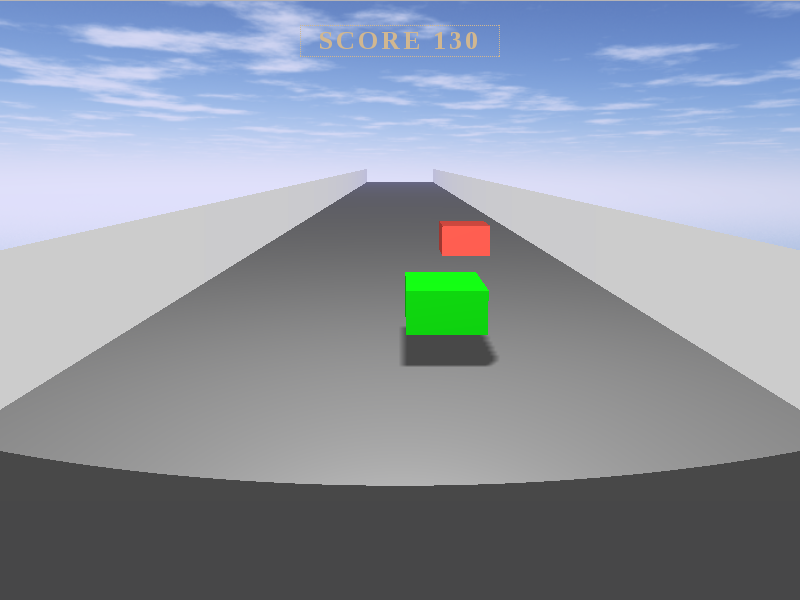
\includegraphics[width=0.8\textwidth,keepaspectratio]{cubes-road-enemy.png}
		\centering
		\caption{Imatge del jugador després d'haver col·lisionat amb varis enemics.}
		\label{fig:cubes-road-enemy}
	\end{figure}
	El moviment horitzontal del cub capturador (verd) es duu a terme mitjançant moviments d'abducció i adducció de la mà.
	\subsubsection{Catch stars - Exercici d'abducció i adducció del dits}
	\subsection{Leap networking plugin}
	\subsection{Aplicació de monitorització}
	Aquesta aplicació permet als responsables de les teràpies de rehabilitació monitoritzar les sessions d'exercicis que fan els seus pacients. D'aquesta manera un responsable pot avaluar la millora d'un pacient. De la mateixa manera es poden detectar errors en la realització dels exercicis.
	
	L'aplicació de monitorització consta de 3 parts fonamentals, un plugin del controlador Leap Motion, un servidor de web socket i una aplicació de reproducció dels moviments capturats pel controlador Leap del pacient. La següent figura mostra un esquema de l'arquitectura de l'aplicació de monitorització.
	\begin{figure}[H]
		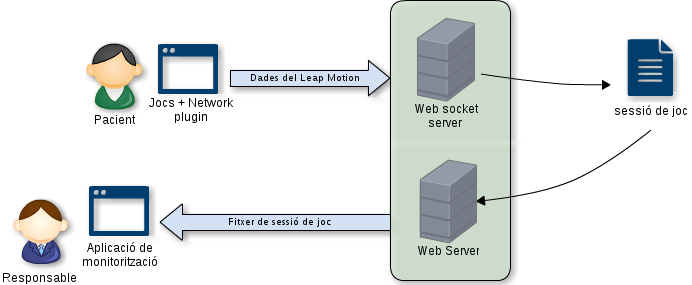
\includegraphics[width=0.8\textwidth,keepaspectratio]{esquema-monitoritzacio.png}
		\centering
		\caption{Arquitectura de l'aplicació de monitorització.}
		\label{fig:arquitectura-monitoritzacio}
	\end{figure}
	Així, un pacient es connecta a un dels jocs definits anteriorment, mentre l'usuari juga, un plugin del Leap Motion va enviantles dades capturades a un servidor de web socket utilitzant una estructura determinada, a la vegada, aquest servidor s'encarrega de guardar les dades rebudes a un fitxer. Després en un altre moment, un dels responsables de la teràpia d'aquest pacient, es connecta a l'aplicació de monitorització per tal de reproduir la sessió de joc del seu pacient. En aquest cas el servidor web l'unic que fa es servir les aplicacions als usuaris i el fitxer de la sessió de joc cap a l'aplicació de monitorització.
	\begin{description}
		\item[Network plugin] aquest és un plugin que segueix la mateixa filosofia que els plugins ja disponibles pel Leap Motion \cite{leapjsplugins}. El primer que fa el plugin és connectar-se a un servidor de web socket. Després quan el controlador Leap Motion comença a enviar dades, aquest plugin les captura i les envia al servidor de socket utilitzant una estructura determinada.
		\item[Web socket] un servidor de web socket tradicional que accepta connexions del plugin del Leap Motion i escolta els esdeveniments d'aquestes connexions. Quan rep una connexió nova, crea un fitxer de text i una vegada creat el fitxer de text, va escrivint les dades rebudes a través del socket al fitxer de text en format JSON. Una vegada que el plugin tanca la connexió amb el servidor, aquest darrer reb un esdeveniment de desconnexió i deixa el fitxer disponible per a ser reproduït per l'aplicació de monitorització.
		\item[GUI de monitorització] és una aplicació web que es connecta al controlador Leap Motion, i utilitza les dades del fitxer, creat per el servidor de socket, per reproduir els moviments de la mà que ha realitzat l'usuari del joc.
		
		Com si es tractàs d'un fitxer de video, aquesta aplicació permet pausar la reproducció dels moviments, així com moure's endavant i enrere. Per tal de facilitar la revisió dels moviments, els usuaris d'aquesta aplicació també tenen la capacitat de rotar la mà que es veu a la reproducció i modificar el zoom de la imatge.
	\end{description}
	\section{Implementació}
	En aquest apartat es descriuen els detalls d’implementació de les diferents aplicacions i sistemes desenvolupats.
	Primer, es presenten les tecnologies utilitzades per desenvolupar les aplicacions i les raons per les quals s’han triat aquestes tecnologies, i després es detallen els aspectes més interessants de la implementació de les diferents aplicacions.
	
	\subsection{Tecnologies utilitzades}
	Durant l’implementació de les aplicacions i sistemes dissenyats s’han utilitzat les següents tecnologies i llenguatges de programació.
	\begin{description}
		\item[HTML, CSS] són la base de l’estructura i el disseny de qualsevol aplicació web.
		\item[JavaScript] és el llenguatge de programació utilitzat pels navegadors web.
		\item[Node.js] és un entorn multiplataforma que permet executar codi JavaScript a la banda del servidor. Presenta una arquitectura basada en esdeveniments i que permet l’execució d’operacions d’entrada i sortida de manera asíncrona. Aquestes prestacions tenen l’objectiu de maximitzar la productivitat d’aplicacions amb múltiples operacions d’entrada i sortida, així com facilitar l’implementació d’aplicacions web de temps real \cite{nodejs}.\\
		Aquestes característiques fan que aquesta tecnologia sigui una de les més adecuades per a la implementació del servidor de web socket, ja que aquesta rebrà moltes peticions i haurà de realitzar operacions d’escritura per a cada petició.
	\end{description}
	\subsection{Detalls d'implementació}
	\section{Futur}
	\section{Conclusions}
	\printbibliography[heading=bibnumbered,title={Bibliografia}]
\end{document}